\subsection{Best Visualization Configurations}
\label{subsec:best-visualization-configs}

The best visualization of the clustering for the mushroom dataset demonstrates two well-separated and compact clusters using kernel PCA reduction, global k-means clustering, and PCA visualization. This result, achieved with the configuration \texttt{pca\_n\_components=3}, \texttt{kernel=rbf}, \texttt{gamma=0.1}, \texttt{n\_clusters=2}, \texttt{max\_iterations=100}, \texttt{tolerance=0.001}, and \texttt{random\_state=4}, effectively highlights the separability of the dataset's two classes in the transformed space.

PCA visualization, especially with Kernel PCA, effectively captures the non-linear relationships in the mushroom dataset by mapping the data into a higher-dimensional space and reducing it to compact, separable clusters. This is well-suited for the mushroom dataset because it has only two distinct classes and exclusively categorical features, making it easier to uncover clear separability in the transformed space.

\begin{figure}[h!]
    \centering
    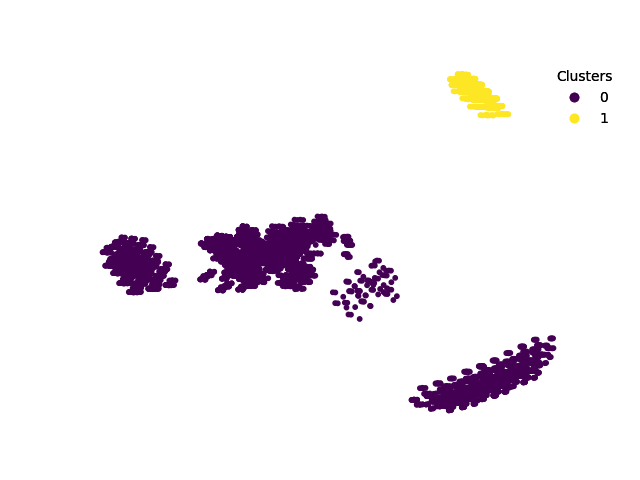
\includegraphics[width=0.8\textwidth]{figures/visualizations/pca_n_components=3,kernel=rbf,gamma=0.1,n_clusters=2,max_iterations=100,tolerance=0.001,random_state=4.png}
    \caption{Clustering visualization for the mushroom dataset using kernel PCA and global k-means clustering.}
    \label{fig:mushroom_clustering}
\end{figure}

The best visualization of the clustering for the vowel dataset is achieved using kernel PCA reduction combined with global k-means clustering and UMAP visualization. This result, obtained with the configuration \texttt{umap\_n\_components=11}, \texttt{kernel=rbf}, \texttt{gamma=1}, \texttt{n\_clusters=11}, \texttt{max\_iterations=100}, \texttt{tolerance=0.0001}, and \texttt{random\_state=4}, effectively captures the dataset's complex structure.

Although the clusters are not as compact as those in the mushroom dataset and often appear as lines rather than blobs, UMAP visualization provides the most interpretable representation for this dataset. The inherent difficulty of finding clear and well-separated clusters is heightened by the presence of 11 natural clusters corresponding to the dataset's diverse vowel classes.

UMAP visualization preserves both local and global structures, which is essential for the vowel dataset due to its high dimensionality and the presence of 11 intricate clusters. Unlike PCA, UMAP can effectively handle the dataset's non-linear relationships and overlapping clusters, revealing patterns that are more interpretable in this complex dataset.

\begin{figure}[h!]
    \centering
    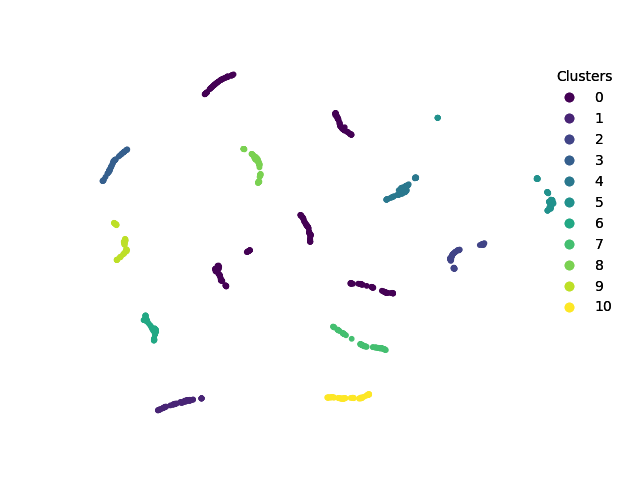
\includegraphics[width=0.8\textwidth]{figures/visualizations/umap_n_components=11,kernel=rbf,gamma=1,n_clusters=11,max_iterations=100,tolerance=0.0001,random_state=4.png}
    \caption{Clustering visualization for the vowel dataset using UMAP and global k-means clustering.}
    \label{fig:vowel_clustering}
\end{figure}
